\documentclass[12pt,a4paper]{report}
\usepackage[utf8]{inputenc}
\usepackage[T1]{fontenc}
\usepackage{babel}
\usepackage{graphicx}
\usepackage{float}
\usepackage[hidelinks]{hyperref}
\usepackage{geometry}
\geometry{margin=1in}
\usepackage{amsmath}
\usepackage{amssymb} % for \checkmark
\usepackage{textcomp} % for \texttimes
\usepackage{array}
\usepackage{longtable}
\usepackage{booktabs}
\usepackage{xcolor}
\usepackage{enumitem}
\usepackage{fancyhdr}
\usepackage[most]{tcolorbox}

% ── Default page style: footer only (line + page number right) ─────────────
\pagestyle{fancy}
\fancyhf{}
\fancyfoot[R]{\thepage}
\renewcommand{\footrulewidth}{0.4pt}
\renewcommand{\headrulewidth}{0pt}

% ── Chapter page style: banner in header + footer ────────────────────────
\fancypagestyle{chapterone}{%
    \fancyhf{}
    % Header: "Chapter 1" italic then full rule
    \fancyhead[L]{%
        \textit{Chapter 1}\\[-4pt]
        \rule{\textwidth}{0.4pt}%
    }
    \renewcommand{\headrulewidth}{0pt}
    % Footer: rule + page number right
    \fancyfoot[R]{\thepage}
    \renewcommand{\footrulewidth}{0.4pt}
}
\fancypagestyle{chaptertwo}{%
    \fancyhf{}
    \fancyhead[L]{%
        \textit{Chapter 2}\\[-4pt]
        \rule{\textwidth}{0.4pt}%
    }
    \renewcommand{\headrulewidth}{0pt}
    \fancyfoot[R]{\thepage}
    \renewcommand{\footrulewidth}{0.4pt}
}
\fancypagestyle{chapterthree}{%
    \fancyhf{}
    \fancyhead[L]{%
        \textit{Chapter 3}\\[-4pt]
        \rule{\textwidth}{0.4pt}%
    }
    \renewcommand{\headrulewidth}{0pt}
    \fancyfoot[R]{\thepage}
    \renewcommand{\footrulewidth}{0.4pt}
}
\fancypagestyle{chapterfour}{%
    \fancyhf{}
    \fancyhead[L]{%
        \textit{Chapter 4}\\[-4pt]
        \rule{\textwidth}{0.4pt}%
    }
    \renewcommand{\headrulewidth}{0pt}
    \fancyfoot[R]{\thepage}
    \renewcommand{\footrulewidth}{0.4pt}
}
\begin{document}

% ==================== TITLE PAGE ====================
\begin{titlepage}
    \thispagestyle{empty}
    \centering

    \begin{minipage}[c]{0.40\linewidth}
        \centering
        
\includegraphics[height=2.0cm]{enicar.jpg}
    \end{minipage}
    \hfill
    \begin{minipage}[c]{0.50\linewidth}
        \raggedleft
        {\small \textbf{National School of Engineers of Carthage}\\[2pt]
        \textsc{ENICarthage --- University of Carthage}}
    \end{minipage}

    \vspace{0.3cm}
    \noindent\rule{\linewidth}{0.4pt}
    \vspace{0.4cm}

    {\normalsize Ministry of Higher Education and Scientific Research\par}

    \vspace{0.5cm}

    {\normalsize \textit{Specialty :}\par}
    {\normalsize Computer Science\par}

    \vspace{0.8cm}

    {\LARGE \textbf{End-of-Studies Project Report}\par}

    \vspace{0.3cm}

    \begin{flushleft}
    {\large \textit{Theme :}\par}
    \end{flushleft}

    {\Large \textbf{\guillemotleft~AI-Powered Automated Penetration Testing~\guillemotright}\par}

    \vspace{1cm}

    {\normalsize \textit{Performed by :}\par}
    \vspace{0.2cm}
    {\large \textbf{Hosni Raissi}\par}

    \vspace{0.8cm}

    {\normalsize \textit{Supervisors :}\par}
    \vspace{0.2cm}
    {\normalsize Mr. Walid Bensa\"{i}d\par}
    {\normalsize Mr. Houcem Hermassi\par}

    \vspace{0.7cm}

    {\normalsize \textit{Work proposed and carried out in collaboration with}\par}
    \vspace{0.5cm}
    
\includegraphics[width=0.28\linewidth]{talan1.png}

    \vspace{0.7cm}

    {\normalsize Academic year : 2025--2026\par}
    \vspace{0.2cm}
    \vfill

    \noindent
    \colorbox{gray!15}{%
        \begin{minipage}{\dimexpr\linewidth}
            \centering
            \vspace{0.25cm}
            {\small National School of Engineers of Carthage\\
            \textbf{ENICarthage}\\
            \textit{45 Avenue des Entrepreneurs, 2035 Charguia II, Tunis-Carthage, Tunisia}\\
            Tel. (+216) 71 941 579 / (+216) 71 940 699 \textendash\ Website: www.enicarthage.rnu.tn}
            \vspace{0.25cm}
        \end{minipage}
    }

\end{titlepage}

% ==================== SIGNATURES ====================
\newpage
\thispagestyle{empty}

{\fontsize{24}{28}\selectfont \textbf{Signatures}}\par

\vspace{0.8cm}

\begin{tcolorbox}[
    enhanced,
    colback=white,
    colframe=black!70,
    boxrule=0.9pt,
    arc=4mm,
    width=\textwidth,
    left=12mm,
    right=12mm,
    top=11mm,
    bottom=11mm
]
I authorize the student to submit the internship report for evaluation.

\vspace{1.1cm}

\centering
Professional Supervisor, \textbf{Mr.\ Walid Bensa\"{i}d}

\vspace{1.6cm}

\begin{flushright}
\textbf{Signature and Stamp}
\end{flushright}
\end{tcolorbox}

\vspace{1.1cm}

\begin{tcolorbox}[
    enhanced,
    colback=white,
    colframe=black!70,
    boxrule=0.9pt,
    arc=4mm,
    width=\textwidth,
    left=12mm,
    right=12mm,
    top=11mm,
    bottom=11mm
]
I authorize the student to submit the internship report for evaluation.

\vspace{1.1cm}

\centering
Academic Supervisor, \textbf{Mr.\ Houcem Hermassi}

\vspace{1.6cm}

\begin{flushright}
\textbf{Signature}
\end{flushright}
\end{tcolorbox}

% ==================== RÉSUMÉ ====================
\newpage
\thispagestyle{fancy}
\section*{R\'{e}sum\'{e}}

Ce travail s'inscrit dans le cadre du projet de fin d'\'{e}tudes de l'\'{E}cole Nationale
d'Ing\'{e}nieurs de Carthage (ENICarthage), en vue de l'obtention du dipl\^{o}me national
d'ing\'{e}nieur en Informatique. Il a \'{e}t\'{e} r\'{e}alis\'{e} lors d'un stage de quatre mois au sein de Talan.
Dans un contexte o\`{u} la surface d'attaque des organisations ne cesse de cro\^{i}tre et o\`{u}
la p\'{e}nurie de professionnels qualifi\'{e}s en cybers\'{e}curit\'{e} constitue un d\'{e}fi structurel,
ce projet propose \textbf{PentaForge} --- une plateforme open-source de tests d'intrusion
automatis\'{e}s, pilot\'{e}e par l'intelligence artificielle. La solution repose sur une
architecture multi-agents organis\'{e}e autour d'un orchestrateur de scan, de n\oe uds
d'information et de m\'{e}moire, ainsi que d'agents sp\'{e}cialis\'{e}s de planification,
reconnaissance, exploitation et analyse. Elle automatise le cycle principal du pentest,
depuis la d\'{e}couverte de la surface d'attaque jusqu'\`{a} la v\'{e}rification et la
structuration des r\'{e}sultats, tout en s'appuyant sur une couche d'ex\'{e}cution isol\'{e}e
pour les outils de s\'{e}curit\'{e}. La plateforme int\`{e}gre \'{e}galement des services
de support pour l'assistance conversationnelle, la synth\`{e}se d'architecture, la
g\'{e}n\'{e}ration de rapports, le partage contr\^{o}l\'{e} de livrables, ainsi que
l'enrichissement des vuln\'{e}rabilit\'{e}s par des scores et vecteurs CVSS. Une couche
de m\'{e}moire et de g\'{e}n\'{e}ration augment\'{e}e par r\'{e}cup\'{e}ration (RAG) am\'{e}liore la
tra\c{c}abilit\'{e} des d\'{e}cisions et la r\'{e}utilisation du contexte projet. La
confidentialit\'{e} des donn\'{e}es client est assur\'{e}e par une couche de sanitisation
appliqu\'{e}e aux \'{e}changes avec les mod\`{e}les de langage, de mani\`{e}re \`{a} anonymiser
ou neutraliser les informations sensibles avant leur transmission.

\vspace{0.4cm}
\noindent \textbf{Mots-cl\'{e}s :} Tests d'intrusion automatis\'{e}s, Intelligence artificielle,
Syst\`{e}me multi-agents, RAG, LLM, CVSS, Cybers\'{e}curit\'{e}, PentaForge.

% ==================== ABSTRACT ====================
\section*{Abstract}

This work is part of the end-of-studies project of the National School of Engineers
of Carthage (ENICarthage), aiming to obtain the national engineering degree in
Computer Science. It was conducted during a four-month internship at Talan.
In a landscape where organizational attack surfaces are expanding rapidly and the
global shortage of qualified cybersecurity professionals creates a structural
imbalance, this project introduces \textbf{PentaForge} --- an open-source, AI-powered
automated penetration testing platform. The solution is built on a multi-agent
architecture centered on a scan orchestrator, deterministic information and memory
nodes, and specialized planner, reconnaissance, exploitation, and analysis agents.
It automates the main penetration testing workflow, from attack-surface discovery to
finding verification and result structuring, while relying on an isolated sandbox
execution layer for security tools. The platform also includes support services for
conversational assistance, architecture synthesis, report generation, controlled
report sharing, and vulnerability enrichment with CVSS vectors and scores. A
Retrieval-Augmented Generation (RAG) and project-memory layer improves decision
traceability and context reuse across the engagement. Client data confidentiality is
enforced through a sanitization layer applied to language-model exchanges, ensuring
that sensitive information is anonymized or neutralized before transmission.

\vspace{0.4cm}
\noindent \textbf{Keywords:} Automated penetration testing, Artificial intelligence,
Multi-agent system, RAG, LLM, CVSS, Cybersecurity, PentaForge.

% ==================== DEDICATIONS ====================
\newpage
\thispagestyle{fancy}
\section*{Dedications}

\vspace{1.2cm}

To my family, unwavering pillar of my life, this work is dedicated to you.
Your love, support, and faith in me have been the foundation of all my successes.

\vspace{1cm}

To my parents, whose wisdom, dedication, and sacrifices have lit every step of my path.
Your unconditional love gave me the strength and determination to overcome every obstacle.

\vspace{1cm}

To my two brothers and my sister, companions at all times, who shared with me
the laughter, the challenges, and the aspirations. Your camaraderie and support
enriched every moment of this adventure.

\vspace{1cm}

To my close friends, who have always been there. Your friendship, encouragement,
and advice played a crucial role in my journey. Your presence and feedback
often guided my choices when it mattered most.

\vspace{1.4cm}

\begin{flushright}
\itshape
To all of you, I dedicate this work as a sign of my deep gratitude\\
and eternal affection.
\end{flushright}

% ==================== ACKNOWLEDGMENTS ====================
\newpage
\thispagestyle{fancy}
\section*{Acknowledgments}

\vspace{1cm}

First and foremost, I wish to express my sincere gratitude to the National School
of Engineers of Carthage (ENICarthage) for the quality of education and the
stimulating academic environment that shaped both my technical and professional path.

\vspace{0.9cm}

I sincerely thank \textbf{Talan} for welcoming me into their team and for providing
me with the opportunity to deepen my knowledge within a demanding professional
environment.

\vspace{0.9cm}

A special thank you to \textbf{Mr.\ Walid Bensaid}, my internship supervisor at Talan,
for his guidance, patience, and invaluable advice throughout this experience.
His support was a constant and decisive source of learning.

\vspace{0.9cm}

I also extend my deepest gratitude to \textbf{Mr.\ Houcem Hermassi} for agreeing
to supervise this work on behalf of ENICarthage. Your advice and recommendations
enlightened my path and were of great help in carrying out this project.

\vspace{0.9cm}

My thanks also go to the \textbf{Talan Cytest team}, whose collaborative spirit,
constructive feedback, and daily commitment were essential to the completion
of this work.

\vspace{0.9cm}

I would like to express my gratitude to the \textbf{members of the jury} for the time
they dedicate to evaluating this work and for their valuable remarks.

\vspace{1.1cm}

\begin{flushright}
\itshape
Finally, I thank all those who, near or far, played a role\\
in my training and in the success of this project.
\end{flushright}

% ==================== TABLE OF CONTENTS ====================
\newpage
\renewcommand{\contentsname}{Table of Contents}
\tableofcontents

% ==================== LIST OF FIGURES ====================
\newpage
\renewcommand{\listfigurename}{List of Figures}
\listoffigures

% ==================== LIST OF TABLES ====================
\newpage
\renewcommand{\listtablename}{List of Tables}
\listoftables

% ==================== ACRONYMS ====================
\newpage
\thispagestyle{fancy}
\section*{Acronyms}
\addcontentsline{toc}{chapter}{Acronyms}

\begin{longtable}{>{\bfseries}p{3.5cm} p{10.5cm}}
\toprule
\textbf{Acronym} & \textbf{Definition} \\
\midrule
\endhead
AI          & Artificial Intelligence \\
API         & Application Programming Interface \\
CISA        & Cybersecurity and Infrastructure Security Agency \\
CISA KEV    & CISA Known Exploited Vulnerabilities \\
CIS         & Center for Internet Security \\
CLI         & Command Line Interface \\
CVE         & Common Vulnerabilities and Exposures \\
CVSS        & Common Vulnerability Scoring System \\
CWE         & Common Weakness Enumeration \\
DAST        & Dynamic Application Security Testing \\
EPSS        & Exploit Prediction Scoring System \\
FP          & False Positive \\
HITL        & Human-in-the-Loop \\
IoC         & Indicator of Compromise \\
IT          & Information Technology \\
JWT         & JSON Web Token \\
LLM         & Large Language Model \\
MITRE ATT\&CK & MITRE Adversarial Tactics, Techniques \& Common Knowledge \\
ML          & Machine Learning \\
MSSP        & Managed Security Service Provider \\
NLP         & Natural Language Processing \\
NVD         & National Vulnerability Database \\
OSINT       & Open Source Intelligence \\
OWASP       & Open Web Application Security Project \\
POC         & Proof of Concept \\
PTES        & Penetration Testing Execution Standard \\
RAG         & Retrieval-Augmented Generation \\
RBAC        & Role-Based Access Control \\
RCE         & Remote Code Execution \\
SARIF       & Static Analysis Results Interchange Format \\
SAST        & Static Application Security Testing \\
SIEM        & Security Information and Event Management \\
SOAR        & Security Orchestration, Automation and Response \\
SSVC        & Stakeholder-Specific Vulnerability Categorization \\
TTP         & Tactics, Techniques and Procedures \\
WAF         & Web Application Firewall \\
\bottomrule
\end{longtable}

% ==================== GENERAL INTRODUCTION ====================
\newpage
\thispagestyle{fancy}
\chapter*{General Introduction}
\addcontentsline{toc}{chapter}{General Introduction}

The rapid expansion of digital infrastructure has fundamentally reshaped the threat
landscape facing organizations of all sizes. Attack surfaces grow faster than security
teams can monitor them, and the global shortage of qualified cybersecurity professionals
creates a structural imbalance that traditional approaches can no longer absorb. In this
context, penetration testing remains one of the most reliable methods for proactively
identifying vulnerabilities before malicious actors exploit them --- yet in its traditional
form, it is slow, manual, fragmented, and difficult to scale.

\vspace{0.8cm}

A standard penetration testing engagement spans between two and six weeks in total —
with active testing typically running one to two weeks and documentation, analysis, and
quality assurance consuming an additional week or more, accounting for roughly a quarter
to a third of the overall engagement time \cite{triaxiomTimeline,valuementorLifecycle}.
Each phase relies on a different set of tools — Nmap, Burp Suite, Metasploit, Nessus —
that operate in isolation and require findings to be transferred manually between them
\cite{autosecagent2026,emazzantiTools}. Context accumulated over hours of work is not
preserved across sessions, causing testers to lose awareness of prior outcomes and
forcing repeated reconstruction of the attack chain \cite{pentestgpt2023}. Retesting
after remediation is rarely exhaustive: industry data suggests that 15 to 25 percent of
remediations contain implementation errors that go undetected \cite{hedgehogRetesting},
and bypass variants of patched vulnerabilities are seldom explored
\cite{redleggRetesting,halockVerification}. These limitations are not the result of poor
practice — they are structural constraints of a fundamentally manual process
\cite{autosecagent2026,cycognitoPentest}.

\vspace{0.8cm}

This project, carried out during a four-month internship at Talan within the Cytest
cybersecurity team, proposes \textbf{PentaForge} as a response to these limitations.
PentaForge is an open-source, AI-assisted penetration testing platform built on a multi
agent architecture designed to support and coordinate the main stages of a security
assessment, including planning, reconnaissance, exploitation support, analysis, and
reporting. The platform combines project memory and retrieval-augmented assistance to
help operators query findings and technical context in natural language, while
maintaining traceability through structured event logging and auditable agent outputs.
Through this approach, PentaForge aims to improve the continuity, efficiency, and
usability of penetration testing workflows while preserving analyst oversight and
technical rigor.

\vspace{0.8cm}

This report is structured around four chapters, organized as follows:

\vspace{0.4cm}

\begin{itemize}
    \setlength{\itemsep}{0.5cm}
    \item \textbf{Chapter 1 --- \guillemotleft~General Framework of the Project~\guillemotright~:}
    Presents the host organization Talan, establishes the project context and problem
    statement, and introduces the development methodology adopted throughout the internship.

    \item \textbf{Chapter 2 --- \guillemotleft~State of the Art~\guillemotright~:}
    Reviews the foundations of AI in cybersecurity and automated penetration testing,
    analyzes existing solutions (PentestGPT, Burp Suite AI, KaliGPT, NodeZero), and
    identifies the gap that PentaForge is designed to fill.

    \item \textbf{Chapter 3 --- \guillemotleft~Specification and Architecture~\guillemotright~:}
    Details the functional and non-functional requirements, presents the global
    four-layer architecture and the deep multi-agent system design, and justifies the
    technical stack choices for both backend and frontend.

    \item \textbf{Chapter 4 --- \guillemotleft~Implementation~\guillemotright~:}
    Covers the concrete realization of the platform, demonstrating the agent
    orchestration cycle, the SSVC classification engine, the RAG chatbot, and the
    end-to-end results produced on a real test environment.
\end{itemize}

\vspace{0.8cm}

This report concludes with a synthesis of the contributions made, the skills acquired
throughout the internship, and the perspectives that could extend PentaForge toward
continuous security validation, automatic threat modeling, and DevSecOps integration.
% ==================== CHAPTER 1 ====================
\newpage
\pagestyle{chapterone}

\vspace*{2cm}

{\fontsize{26}{30}\selectfont \textbf{Chapter 1}}\par

\vspace{1cm}

{\LARGE\bfseries General Framework of the Project}

\vspace{0.8cm}

\addcontentsline{toc}{chapter}{Chapter 1 --- General Framework of the Project}
\setcounter{chapter}{1}
\setcounter{section}{0}

\section*{Introduction}
\addcontentsline{toc}{section}{Introduction}

This chapter serves to anchor the project in its overall framework. We begin by
presenting Talan, the company that hosted this internship, before examining the
specific context and structural challenges that motivated PentaForge, and finally
detailing the Scrum development methodology adopted throughout the project.
% ── Section 1 ─────────────────────────────────────────────────────────────
\section{Presentation of the Company Talan}

\subsection{About Talan}

Founded in 2002 by Philippe Cassoulat, Mehdi Houas, and Eric Benamou, Talan is a
French IT consulting and services company. Present in Tunisia since 2008, the group
quickly expanded internationally, now covering five continents and many countries such
as Canada, Spain, the United States, Belgium, Luxembourg, the United Kingdom, and
Switzerland.

Talan today has nearly 6,000 employees worldwide. Talan's mission is to advise
companies and public administrations, assist them, and implement their transformation
projects. Constantly evolving, the group specializes in future-oriented fields such as
Big Data, IoT, Blockchain, and Artificial Intelligence, to meet the needs of its most
demanding clients.

Talan Tunisie Consulting is Talan's ``Nearshore'' development center, based in Tunis
since 2008. This subsidiary brings together more than 500 engineers specialized in new
technology development. They work for major European clients and come from the top
Tunisian and European engineering schools. Thanks to their expertise, Talan Tunisie
Consulting offers tailor-made solutions to support its clients in their digital
transformation.

\begin{figure}[H]
    \centering
    
\includegraphics[width=0.3\textwidth]{talan1.png}
    \caption{Talan Logo}
    \label{fig:logo_talan}
\end{figure}

\subsection{Services Offered by Talan}

Talan offers a complete range of services to support its clients in their digital
and technological projects:

\begin{itemize}
    \item \textbf{Digital:} Development of web and mobile solutions, including the
    establishment of offshore service centers and digital transformation.
    \item \textbf{Integration:} Implementation of CRM, ERP, middleware solutions,
    as well as BI and DATA solutions.
    \item \textbf{Testing:} Supporting clients in implementing testing methodologies,
    executing manual tests, test automation, and third-party testing.
    \item \textbf{Support:} Level 2 and 3 application and functional support,
    monitoring of business applications in production, management of developments,
    and continuous improvement.
    \item \textbf{Innovation Factory:} Talan's research and development center,
    focused on disruptive technologies to deliver added value.
    \item \textbf{Cyber Security:} Consulting in cybersecurity, compliance, and
    governance, penetration testing, and security audits.
\end{itemize}

\subsection{Talan's Area of Expertise}

Talan Tunisie Consulting has extensive expertise in several areas, including
consulting, assistance, project management, integration of new technologies, and
support services related to information systems. Its areas of intervention include:

\begin{itemize}
    \item \textbf{Finance:} Collaboration with large financial institutions, including
    investment banks and asset managers.
    \item \textbf{Telecom:} Growing involvement in the telecom sector, providing
    innovative solutions to major operators.
    \item \textbf{Transport and Logistics:} Born from the merger with Cereza in 2012,
    the department's mission is to support players in their optimization and
    transformation projects.
    \item \textbf{Insurance:} Deep expertise in the insurance sector, allowing to
    address specific issues such as regulation or asset management.
    \item \textbf{Energy and Environment:} A major player in the energy sector,
    anticipating market developments and managing information system challenges.
\end{itemize}

% ── Section 2 ─────────────────────────────────────────────────────────────
\section{Project Context}

\subsection{Problem Statement}

Penetration testing remains one of the most reliable methods for proactively
identifying vulnerabilities in an organization's information systems before malicious
actors can exploit them. However, in its traditional form, it suffers from structural
limitations that prevent it from scaling to meet the demands of modern IT environments.

A standard engagement typically spans two to six weeks in total --- with active
testing representing one to two weeks of that period and documentation, analysis,
and quality assurance consuming an additional week or more, accounting for roughly
a quarter to a third of the overall effort~\cite{triaxiomTimeline,valuementorLifecycle}. Each phase of the
lifecycle relies on a different set of specialized tools --- Nmap, Burp Suite,
Metasploit, Nessus --- that operate in isolation and require findings to be
transferred manually between them~\cite{autosecagent2026,emazzantiTools}. Context accumulated over
hours of work is not preserved across sessions, causing testers to lose awareness
of prior outcomes and forcing repeated reconstruction of the attack
chain~\cite{pentestgpt2023}. Retesting after remediation is rarely exhaustive: studies
suggest that a significant proportion of remediations contain implementation
errors that go undetected~\cite{hedgehogRetesting}, and bypass variants of patched
vulnerabilities are seldom explored~\cite{redleggRetesting,halockVerification}. These limitations are
not the result of poor practice --- they are structural constraints of a
fundamentally manual process~\cite{autosecagent2026,cycognitoPentest}.

Beyond these operational challenges, the global shortage of qualified cybersecurity
professionals means that many organizations cannot sustain the testing frequency
their attack surface demands. Manual penetration testing does not scale --- a
single expert can only effectively cover a limited number of targets
simultaneously, and faced with a cloud infrastructure comprising hundreds of
services, manual methods become structurally insufficient.

\subsection{Proposed Solution}

To address these structural limitations, this project introduces \textbf{PentaForge}
--- an open-source, AI-assisted penetration testing platform built on a multi-agent
architecture. Rather than replacing the security professional, PentaForge is designed
to augment their capabilities by automating repetitive and time-consuming tasks while
preserving human control over high-impact security decisions.

The platform coordinates a set of specialized AI agents --- Planner, Executer,
and Analyzer --- that support the main phases of a penetration testing workflow,
including reconnaissance, execution, analysis, and reporting. A persistent
\textbf{System Memory} layer helps preserve context across sessions by maintaining
an updated view of the target profile, findings, and execution history. A
\textbf{Retrieval-Augmented Generation (RAG)} knowledge base helps keep the
platform's security intelligence current without retraining the underlying model.
A built-in \textbf{Assistant Agent} enables pentesters and analysts to query
findings and project context in natural language throughout the engagement.
Finally, a \textbf{Verification Tier} mechanism requires structured validation
before a finding is classified as confirmed, thereby reducing the risk of unreliable
or hallucinated outputs.

It is therefore important to clarify that PentaForge is not intended to replace the
full work of a penetration tester. Its role is to assist the analyst by accelerating
technical tasks, preserving context, and surfacing possible vulnerabilities or attack
paths that still require professional interpretation, validation, and decision-making
before they can be treated as reliable security conclusions.

By adopting this approach, PentaForge aims to reduce repetitive manual effort,
preserve engagement continuity across sessions, and make penetration testing more
scalable without removing analyst oversight from sensitive security decisions.

\subsection{Target Audience}

PentaForge is designed for security professionals and organizations that require
systematic, repeatable, and scalable penetration testing. Its primary users include:

\begin{itemize}
    \item \textbf{Penetration testers and red teams,} who benefit from workflow
    assistance in reconnaissance, execution support, evidence collection, and
    reporting, freeing them to focus on creative, high-judgment attack paths.

    \item \textbf{Security managers and decision-makers,} who need clear visibility
    into findings, project status, and generated security outputs without requiring
    deep technical expertise.

    \item \textbf{Managed Security Service Providers (MSSPs),} who seek to improve
    engagement efficiency and handle a larger volume of assessments with better
    operational continuity.

    \item \textbf{Organizations with large or evolving attack surfaces,} such as
    technology companies, cloud-oriented environments, and complex enterprise
    infrastructures where manual testing frequency is insufficient.

    \item \textbf{Institutions with strict confidentiality or governance
    requirements,} where traceability, controlled execution, and local handling
    of sensitive project data are non-negotiable.
\end{itemize}

\subsection{Scrum Development Methodology}

We adopted the \textbf{Scrum} agile methodology to manage the development of
PentaForge. Given the exploratory nature of an AI-driven platform --- where agent
behavior, tool integration results, and LLM output quality are only fully understood
through iterative testing --- a methodology that embraces continuous feedback and
incremental delivery was essential.

Scrum organizes development into fixed-length \textbf{sprints} of two weeks each.
At the start of each sprint, a planning session defines the backlog items to be
delivered. A daily stand-up ensures coordination and surfaces blockers early. At the
end of each sprint, a review demonstrates the working increment to stakeholders, and
a retrospective identifies process improvements for the next cycle. The four Scrum
ceremonies applied throughout this project were:

\begin{enumerate}
    \item \textbf{Sprint Planning:} Definition of sprint goals and selection of
    backlog items based on priority and team capacity.
    \item \textbf{Daily Stand-up:} Brief daily synchronization on progress,
    plans, and impediments.
    \item \textbf{Sprint Review:} Demonstration of the completed increment and
    collection of feedback from the Talan Cytest team.
    \item \textbf{Sprint Retrospective:} Reflection on the development process
    to continuously improve team efficiency and delivery quality.
\end{enumerate}

\begin{figure}[H]
    \centering
    % \includegraphics[width=0.8\textwidth]{scrum_process.png}
    \caption{Scrum Development Process}
    \label{fig:scrum}
\end{figure}

\subsection{Project Planning}

The project was carried out over a period of four months, organized into six
two-week sprints:

\begin{enumerate}
    \item \textbf{Sprint 1 --- Knowledge Infrastructure \& Intel Agent (Weeks 1--2)}
    \begin{itemize}
        \item Set up the core persistence stack: Projects Store, Redis, Qdrant,
        Intel state tracking, and filesystem-backed artifact storage
        \item Build the RAG embedding pipeline with per-domain vector indexes
        \item Implement the Intel Agent to ingest NVD, CISA KEV, and ExploitDB feeds
    \end{itemize}

    \item \textbf{Sprint 2 --- Scope \& Safety Engine + Planner Agent (Weeks 3--4)}
    \begin{itemize}
        \item Implement the Scope Enforcer, Rate Limiter, Kill Switch, and
        Prompt Injection Guard
        \item Build the Planner with Fast Path (PTES state machine) and
        Slow Path (LLM Chain-of-Thought)
        \item Implement the ActionPlan JSON schema and the World State feedback loop
    \end{itemize}

    \item \textbf{Sprint 3 --- Executor Agents \& Tool Abstraction Registry (Weeks 5--6)}
    \begin{itemize}
        \item Implement the Tool Abstraction Registry with context-aware tool selection
        \item Build and integrate the Recon, Exploit, Verify, Report, and Retest agents
        \item Validate the end-to-end scan chain on a local lab environment
    \end{itemize}

    \item \textbf{Sprint 4 --- Compensator \& Perceptor (Weeks 7--8)}
    \begin{itemize}
        \item Implement agent fault isolation, state checkpointing, and recovery
        \item Build the SSVC classification pipeline integrating CVSS, EPSS,
        CISA KEV, and asset context
        \item Integrate the Perceptor output parsers for all executor agents
    \end{itemize}

    \item \textbf{Sprint 5 --- Interface Layer \& HITL Chatbot (Weeks 9--10)}
    \begin{itemize}
        \item Build the FastAPI backend with RBAC and JWT authentication
        \item Implement the live dashboard, Approval Gate, and RAG chatbot interface
        \item Develop the client portal with scoped access and on-demand report export
    \end{itemize}

    \item \textbf{Sprint 6 --- Integration, Hardening \& Packaging (Weeks 11--12)}
    \begin{itemize}
        \item Run a full end-to-end engagement on a multi-target lab environment
        \item Apply security hardening: secrets management, prompt injection
        regression testing, and RBAC boundary audit
        \item Package the platform with Docker Compose for single-command deployment
    \end{itemize}
\end{enumerate}

\section*{Conclusion}
\addcontentsline{toc}{section}{Conclusion}

This first chapter has established the general framework of the internship at Talan,
identified the structural limitations of traditional penetration testing that motivated
this project, and introduced PentaForge as the proposed solution. The Scrum methodology
and six-sprint roadmap provide a clear and iterative execution plan for the twelve
weeks of development ahead.

The next chapter examines the state of the art --- exploring the role of artificial
intelligence in cybersecurity, the current landscape of automated penetration testing
tools, and the specific gap that PentaForge is designed to fill.

% ── Restore default page style for subsequent chapters ─────────────────────
\pagestyle{fancy}
% ==================== CHAPTER 2 ====================
\newpage
\pagestyle{chaptertwo}

\vspace*{4cm}

{\fontsize{26}{30}\selectfont \textbf{Chapter 2}}\par

\vspace{1cm}

{\LARGE\bfseries State of the Art}

\vspace{0.8cm}

\addcontentsline{toc}{chapter}{Chapter 2 --- State of the Art}
\setcounter{chapter}{2}
\setcounter{section}{0}

\section*{Introduction}
\addcontentsline{toc}{section}{Introduction}

This chapter establishes the theoretical and technical foundations upon which
PentaForge is built. We begin by examining the role of artificial intelligence
in cybersecurity, surveying the principal use cases where machine learning and
large language models have transformed defensive and offensive security practices.
We then focus specifically on the penetration testing domain, describing the
traditional lifecycle and the points where AI can intervene most effectively.
Finally, we conduct a comparative analysis of existing automated penetration
testing solutions, identifying the gap in the current landscape that motivates
the design choices of PentaForge.

% ── Section 1 ─────────────────────────────────────────────────────────────
\section{Artificial Intelligence in Cybersecurity}

\subsection{General Context}

The cybersecurity landscape is undergoing a profound structural transformation.
The explosion in the number of connected systems, the growing sophistication of
attackers, and the global shortage of qualified professionals create a structural
imbalance between the attack surface and the defensive capabilities of organizations.
Faced with this reality, artificial intelligence is emerging as the technological
lever capable of restoring this balance.

AI does not replace the security expert --- it multiplies their capabilities. It
automates repetitive low-value tasks, detects patterns invisible to the human eye,
and operates at a speed and scale inaccessible to a single analyst.

\subsection{Threat Detection and Anomaly Detection}

Next-generation SIEM (Security Information and Event Management) systems integrate
machine learning models to detect abnormal behavior in real time. Where static rules
fail against zero-day attacks, supervised and unsupervised models identify statistical
deviations from the normal behavior of a network. Key techniques include:

\begin{itemize}
    \item \textbf{UEBA (User and Entity Behavior Analytics):} detection of suspicious
    lateral movements through behavioral baseline modeling.
    \item \textbf{Time series models:} identification of nocturnal data exfiltration
    patterns that evade signature-based detection.
    \item \textbf{Unsupervised clustering:} grouping of unknown indicators of
    compromise into actionable threat families.
    \item \textbf{NLP on logs:} semantic correlation between dispersed events across
    heterogeneous log sources.
\end{itemize}

\subsection{Malware Analysis}

Static and dynamic malware analysis directly benefits from AI. Binary code
classification models automatically categorize malware families without prior
signatures. Architectures such as Graph Neural Networks (GNN) analyze system call
graphs to detect obfuscated malicious behavior that would be invisible to
traditional antivirus engines.

\subsection{Automated Threat Intelligence}

AI enables the automatic processing and correlation of threat intelligence (CTI)
feeds from multiple sources: NVD, CISA KEV, ExploitDB, and threat actor reports.
Natural Language Processing (NLP) extracts Indicators of Compromise (IoC) from
unstructured reports, enabling security teams to operationalize intelligence at
a speed and scale that manual analysis cannot match.

\subsection{Incident Response and SOAR}

SOAR (Security Orchestration, Automation and Response) platforms integrate AI
agents capable of automatically triggering response playbooks. When a ransomware
alert is detected, an AI agent can isolate the affected machine within seconds ---
well before a human analyst has had time to read the notification. Reinforcement
learning enables these agents to improve their response strategies over time based
on outcome feedback.

\subsection{Application Security}

AI-augmented static code analysis (SAST) identifies vulnerabilities in source code
with fewer false positives than traditional rule-based tools. Large Language Models
(LLM) are now capable of explaining a vulnerability, generating a proof-of-concept
exploit, and proposing a remediation fix --- all within an automated pipeline. This
capability is central to the design of PentaForge's Exploit and Report agents.

\begin{table}[H]
    \centering
    \caption{AI application domains in cybersecurity}
    \label{tab:ai_domains}
    \renewcommand{\arraystretch}{1.3}
    \begin{tabular}{lll}
        \toprule
        \textbf{Domain} & \textbf{AI Technique} & \textbf{Key Advantage} \\
        \midrule
        Intrusion Detection  & Anomaly detection, LSTM        & Real-time, zero-day   \\
        Malware Analysis     & CNN, GNN, classification       & Signature-free        \\
        Threat Intelligence  & NLP, NER, clustering           & Auto-correlation      \\
        Automated Pentest    & LLM, multi-agent systems       & Scalability, speed    \\
        SOAR                 & Reinforcement Learning         & Autonomous response   \\
        SAST/DAST            & Transformers, RAG              & Fewer false positives \\
        \bottomrule
    \end{tabular}
\end{table}

% ── Section 2 ─────────────────────────────────────────────────────────────
\section{AI in Penetration Testing}

\subsection{The Traditional Penetration Testing Lifecycle}

A penetration test follows a structured methodology defined by the PTES
(Penetration Testing Execution Standard) and aligned with the MITRE ATT\&CK
framework. This cycle comprises five fundamental phases:

\begin{enumerate}
    \item \textbf{Reconnaissance} --- passive and active collection of information
    about the target: open ports, exposed services, technology stack, and
    organizational footprint.
    \item \textbf{Scanning \& Enumeration} --- mapping of services, port states,
    software versions, and potential entry points.
    \item \textbf{Exploitation} --- controlled attempts to exploit identified
    vulnerabilities to confirm their real-world impact.
    \item \textbf{Post-Exploitation} --- privilege escalation, lateral movement,
    persistence mechanisms, and data exfiltration simulation.
    \item \textbf{Reporting} --- documentation of findings, evidence, severity
    ratings, and remediation recommendations.
\end{enumerate}

Executed manually, this cycle takes an average of two to four weeks for a standard
engagement. AI allows this timeframe to be compressed to a few hours for the
majority of automatable phases.

\subsection{AI Intervention Points in the Pentest Lifecycle}

\subsubsection{Automatic Generation of Attack Scenarios}

LLMs are capable of generating complex attack scenarios from a description of the
target. Drawing on their knowledge of the MITRE ATT\&CK framework and documented
TTPs (Tactics, Techniques, and Procedures), they produce multi-step attack plans
--- coherent attack chains that simulate the behavior of a real attacker. This
capability forms the core of the Planner agent in PentaForge.

\subsubsection{Adaptive Payload Generation}

LLMs generate payloads adapted to the target context --- WAF profile, detected
technologies, and filter behavior. This contextual generation far exceeds the
capabilities of static wordlists used by traditional tools, enabling techniques
such as dynamic WAF bypass encoding, DBMS-specific SQL injection variants, and
context-aware XSS payloads.

\subsubsection{Intelligent Classification and False Positive Filtering}

Managing false positives represents one of the highest costs in penetration testing.
A classic scanner can generate hundreds of alerts, 40 to 60\% of which are false
positives. AI significantly reduces this ratio by using classification models
trained on real vulnerability databases, computer vision to visually validate POC
screenshots, and behavioral analysis of the application response to confirm
exploitability.

\subsubsection{Automated Evidence Capture}

Evidence documentation is a time-consuming but critical task. AI automates
screenshot capture at the precise moment of exploitation, visual annotation using
a vision model, SHA-256 hashing to guarantee forensic integrity, and automatic
construction of an evidence chain linking each finding to its proof of concept.

\subsubsection{Automated Retest After Remediation}

After a client has deployed a fix, manual retesting is tedious and often incomplete.
An AI agent can automatically replay original payloads, generate mutations to test
bypasses, and compare before-and-after responses to produce a confidence score on
the effectiveness of the patch.

\subsubsection{Conversational Interface on Reports}

A RAG (Retrieval-Augmented Generation) chatbot allows pentesters, CISOs, and
analysts to query results in natural language. This interface transforms a static
report into an interactive knowledge base accessible to both technical and
non-technical stakeholders.

\begin{table}[H]
    \centering
    \caption{Estimated gains brought by AI to the pentest lifecycle}
    \label{tab:ai_gains}
    \renewcommand{\arraystretch}{1.3}
    \begin{tabular}{lll}
        \toprule
        \textbf{Phase}    & \textbf{AI Contribution}              & \textbf{Estimated Gain} \\
        \midrule
        Reconnaissance    & Multi-source OSINT automation         & $-70\%$ time            \\
        Scanning          & Intelligent target prioritization     & $-50\%$ noise           \\
        Exploitation      & Contextual payload generation         & $+40\%$ coverage        \\
        Evidence          & Automatic capture and annotation      & $-80\%$ effort          \\
        Classification    & AI false positive filtering           & $-60\%$ false positives \\
        Reporting         & Automatic PDF/HTML/SARIF generation   & $-90\%$ time            \\
        Retest            & Automatic replay and mutation         & $-85\%$ effort          \\
        \bottomrule
    \end{tabular}
\end{table}

% ── Section 3 ─────────────────────────────────────────────────────────────
\section{Existing Solutions and Comparative Analysis}

\subsection{PentestGPT}

PentestGPT is an open-source solution that integrates an LLM into a pentester's
workflow via a CLI interface. Its architecture is based on a three-module reasoning
loop: a Reasoning Module for strategic planning, a Generation Module for command
and payload generation, and a Parsing Module for analyzing tool outputs and feeding
results back to the reasoning layer.

\textbf{Strengths:} context maintenance over long sessions, support for local LLMs
via Ollama, and multi-category coverage across web, crypto, forensics, and privilege
escalation scenarios.

\textbf{Limitations:} no automatic POC capture, no intelligent false positive
filtering, no retest automation, no conversational interface on reports, and a
monolithic architecture with no agent parallelization.

\subsection{Burp Suite AI (PortSwigger)}

Burp Suite Pro integrates advanced AI features for web application penetration
testing. Its Explore Issue model detects a vulnerability, attempts real exploitation,
and generates a functional proof of concept with a step-by-step log. An LSTM-based
adaptive learning model reduces false positives by modeling application behavior
over time.

\textbf{Strengths:} real exploitation confirmation with automated POC generation,
effective false positive reduction, and an MCP architecture that exposes pentest
capabilities to external AI agents.

\textbf{Limitations:} exclusively focused on web applications with no network,
cloud, or infrastructure coverage; human-first philosophy prevents autonomous
operation; no chatbot interface for querying historical reports; and a costly
commercial license.

\subsection{KaliGPT}

KaliGPT integrates an LLM into Kali Linux, allowing execution and analysis of
penetration testing commands via a structured workflow. Its \texttt{run} pattern
automatically routes each tool execution through AI analysis without requiring
manual copy-paste.

\textbf{Strengths:} elegant command analysis pattern, and a structured workflow
covering the complete cycle from reconnaissance to reporting.

\textbf{Limitations:} no state persistence between sessions, sequential execution
only with no parallel agents, no scope management or rules of engagement, and no
automatic structured report generation.

\subsection{NodeZero (Horizon3.ai)}

NodeZero is a commercial SaaS autonomous penetration testing platform representing
the enterprise state of the art. It delivers end-to-end automation, multi-surface
coverage, impact-based prioritization, and executive reporting.

\textbf{Strengths:} the most complete automation available commercially, with
persistent context and prioritized findings.

\textbf{Limitations:} closed SaaS model with no possible customization, no
on-premise deployment option, prohibitive cost for most organizations, and no
open-source access for research or adaptation.

\subsection{Comparative Matrix}

Table~\ref{tab:comparison} summarizes the coverage of each solution across the
criteria most relevant to PentaForge's design goals.

\begin{table}[H]
    \centering
    \caption{Comparative analysis of existing automated penetration testing solutions}
    \label{tab:comparison}
    \renewcommand{\arraystretch}{1.4}
    \begin{tabular}{lccccc}
        \toprule
        \textbf{Criterion}     & \textbf{PentestGPT} & \textbf{Burp AI} & \textbf{KaliGPT} & \textbf{NodeZero} & \textbf{PentaForge} \\
        \midrule
        Parallel agents        & \texttimes & \texttimes & \texttimes & \checkmark & \checkmark \\
        Auto POC capture       & \texttimes & \checkmark & \texttimes & \checkmark & \checkmark \\
        AI FP filtering        & \texttimes & \checkmark & \texttimes & \checkmark & \checkmark \\
        Automated retest       & \texttimes & \texttimes & \texttimes & $\approx$  & \checkmark \\
        RAG chatbot            & \texttimes & \texttimes & \texttimes & \texttimes & \checkmark \\
        Explainability         & \texttimes & $\approx$  & \texttimes & $\approx$  & \checkmark \\
        Multi-surface          & \checkmark & \texttimes & \checkmark & \checkmark & \checkmark \\
        Open source            & \checkmark & \texttimes & \checkmark & \texttimes & \checkmark \\
        On-premise             & \checkmark & $\approx$  & \checkmark & \texttimes & \checkmark \\
        Kill Switch            & \texttimes & \texttimes & \texttimes & $\approx$  & \checkmark \\
        Persistent World State & \texttimes & $\approx$  & \texttimes & \checkmark & \checkmark \\
        \bottomrule
        \multicolumn{6}{l}{\small \checkmark~Present \quad $\approx$~Partial \quad \texttimes~Absent}
    \end{tabular}
\end{table}

\subsection{Identified Gap and PentaForge's Position}

The comparative analysis reveals a value space unaddressed by existing solutions:
an open-source, on-premise, multi-agent platform that combines all the following
properties simultaneously --- parallel agent execution, persistent engagement
context, automated retest with bypass detection, full explainability of agent
decisions, and a RAG-powered conversational interface.

PentestGPT and KaliGPT are open-source but lack parallelism, persistence, and
automation. Burp Suite AI offers strong false positive filtering but is limited
to web applications and requires a commercial license. NodeZero delivers the most
complete automation but is a closed, expensive SaaS with no customization or
on-premise option.

PentaForge is designed to occupy the intersection of these two axes: the openness
and customizability of PentestGPT with the automation depth of NodeZero, deployable
entirely on-premise with no data leaving the engagement perimeter.

% ── Section 4 ─────────────────────────────────────────────────────────────
\section{Key Technologies Underpinning PentaForge}

\subsection{Large Language Models and Chain-of-Thought Reasoning}

Large Language Models (LLMs) are transformer-based neural networks trained on
large text corpora that have demonstrated remarkable capabilities in code generation,
reasoning, and structured output production. For penetration testing, LLMs provide
the strategic reasoning layer --- the ability to read a target profile, consult a
knowledge base, and produce a structured attack plan with explicit dependency chains
and fallback strategies.

Chain-of-Thought (CoT) prompting enables the LLM to reason step-by-step before
producing its output, significantly improving the quality and coherence of generated
attack plans for novel or complex targets. PentaForge's Planner uses CoT reasoning
in its Slow Path for engagements that fall outside standard PTES templates.

\subsection{Retrieval-Augmented Generation}

Retrieval-Augmented Generation (RAG) addresses a fundamental limitation of LLMs:
their knowledge is frozen at training time. In a cybersecurity context where new
CVEs are published daily and attack techniques evolve continuously, a frozen model
is a liability.

RAG decouples knowledge from model weights. When an agent needs domain-specific
guidance --- exploit techniques for a specific CVE, WAF bypass patterns for a
detected technology, or compliance mappings for a finding --- it performs a vector
similarity search over a continuously updated knowledge base (Qdrant in
PentaForge) and injects the retrieved context directly into the prompt. This
ensures the platform's knowledge is always current without requiring model
retraining.

\subsection{Multi-Agent Systems}

A multi-agent system (MAS) is an architecture in which multiple autonomous agents,
each with a specialized role and capability set, collaborate to achieve a goal that
no single agent could accomplish alone. In the penetration testing domain, this
specialization is natural: reconnaissance, exploitation, verification, and reporting
require fundamentally different tool sets, reasoning strategies, and output formats.

The key properties of an effective MAS for penetration testing are: agent
parallelism (multiple agents working simultaneously on independent targets),
shared state (a common knowledge base that all agents read from and write to),
fault isolation (a crashed agent does not block the entire pipeline), and
orchestration (a coordinator that resolves dependencies and sequences tasks
based on current knowledge).

\subsection{SSVC --- Stakeholder-Specific Vulnerability Categorization}

The Common Vulnerability Scoring System (CVSS) provides a severity score for
vulnerabilities in isolation, without regard to the specific environment in which
they exist. A CVSS 9.8 vulnerability on an air-gapped test server is far less
urgent than a CVSS 6.5 vulnerability on an internet-facing payment API.

SSVC (Stakeholder-Specific Vulnerability Categorization), developed by CISA and
Carnegie Mellon University, addresses this limitation by incorporating four
contextual dimensions into the prioritization decision: exploitation state (from
NVD and CISA KEV), technical impact (from CVSS), automatable exploitation
likelihood (from EPSS), and mission prevalence (from the asset inventory). The
output is a decision --- ACT, ATTEND, or TRACK --- rather than a score, providing
security teams with actionable guidance rather than a number to interpret.

\section*{Conclusion}
\addcontentsline{toc}{section}{Conclusion}

This chapter has established the theoretical foundations of PentaForge by surveying
the role of AI in cybersecurity, the state of automated penetration testing, and the
limitations of existing solutions. The comparative analysis confirms that no current
open-source tool combines parallel multi-agent execution, persistent engagement
context, automated retest with bypass detection, full explainability, and a
RAG-powered conversational interface in a single on-premise platform.

The technologies reviewed in the final section --- LLMs with Chain-of-Thought
reasoning, Retrieval-Augmented Generation, multi-agent architectures, and SSVC
classification --- collectively form the technical foundation of PentaForge's design.
The following chapter translates these foundations into a concrete specification and
architecture for the platform.

% ── Restore default page style for subsequent chapters ─────────────────────
\pagestyle{fancy}
% ==================== CHAPTER 3 ====================
\newpage
\pagestyle{chapterthree}

\vspace*{4cm}

{\fontsize{26}{30}\selectfont \textbf{Chapter 3}}\par

\vspace{1cm}

{\LARGE\bfseries Specification and Architecture}

\vspace{0.8cm}

\addcontentsline{toc}{chapter}{Chapter 3 --- Specification and Architecture}
\setcounter{chapter}{3}
\setcounter{section}{0}

\section*{Introduction}
\addcontentsline{toc}{section}{Introduction}

This chapter translates the theoretical foundations established in Chapter 2 into
the concrete specification and architectural design of PentaForge as it exists in
the implemented project. The objective is not to describe a hypothetical platform,
but to formalize the current product structure, its actors, the responsibilities of
each subsystem, and the technical rationale behind its organization. We first
identify the actors and requirements that shape the platform. We then present the
global architecture, detail the multi-agent execution loop together with the support
services that surround it, and conclude with the technical stack retained for the
desktop client, backend services, storage layer, and sandboxed execution path.

% ── Section 1 ─────────────────────────────────────────────────────────────
\section{Requirements Analysis}

\subsection{Platform Actors}

PentaForge is designed around three operational actors whose responsibilities are
clearly separated in the current product workflow.

\begin{table}[H]
    \centering
    \caption{PentaForge actors and their responsibilities}
    \label{tab:actors}
    \renewcommand{\arraystretch}{1.4}
    \begin{tabular}{lll}
        \toprule
        \textbf{Actor}       & \textbf{Profile}            & \textbf{Rights and Responsibilities} \\
        \midrule
        Pentester            & Technical operator          & Creates projects, defines target     \\
                             &                             & type and target metadata, launches   \\
                             &                             & scans, approves sensitive actions,   \\
                             &                             & reviews findings and exports reports \\
        \midrule
        Client               & External stakeholder        & Accesses a scoped delivery portal,   \\
                             &                             & reviews reports, receives share      \\
                             &                             & links, and exchanges messages with   \\
                             &                             & the pentester                        \\
        \midrule
        Administrator        & Platform maintainer         & Manages target-type schemas,         \\
                             &                             & information-gathering profiles,      \\
                             &                             & LLM settings, Intel resources, and   \\
                             &                             & deployment/runtime configuration     \\
        \bottomrule
    \end{tabular}
\end{table}

\subsection{Functional Requirements}

The functional requirements define the concrete capabilities currently expected from
PentaForge. They are organized around the four major operational responsibilities of
the platform.

\textbf{Project and Scope Management}
\begin{itemize}
    \item The system shall allow the pentester to create a project, select a target
    type, and provide structured target information adapted to that type.
    \item The system shall support multiple target categories such as web
    applications, APIs, infrastructure, networks, cloud, mobile, IoT, containers,
    repositories, and Linux servers.
    \item The system shall persist the complete project state, including target
    metadata, scan state, reports, findings, and delivery information.
    \item The system shall maintain editable information-gathering profiles for each
    target type so that reconnaissance baselines remain configurable from the UI.
\end{itemize}

\textbf{Supervised Scan Orchestration}
\begin{itemize}
    \item The system shall launch a scan from a project and preserve the operational
    context of that scan in a dedicated runtime state.
    \item The system shall execute the early scan phases through deterministic and
    agent-assisted services, beginning with Intel and warmup reconnaissance.
    \item The system shall stream live scan events to the frontend so the operator
    can follow progress, approvals, warnings, and results in real time.
    \item The system shall support operator approval workflows for planning changes,
    information-gathering steps, sensitive tools, and password-dependent actions.
    \item The system shall expose a pause or cancel mechanism for long-running scans.
\end{itemize}

\textbf{Analysis, Reporting, and Delivery}
\begin{itemize}
    \item The system shall preserve verified and unverified findings in project
    storage and prepare them for analyst and report workflows.
    \item The system shall generate operator-facing reports in Markdown and HTML,
    with PDF export produced on demand from the report path.
    \item The system shall provide protected delivery links so that a client can
    access the report in a scoped portal without direct access to scan controls.
    \item The system shall support password-protected report export packages for
    secure transfer outside the platform.
\end{itemize}

\textbf{Assistant and Execution Support}
\begin{itemize}
    \item The system shall provide an assistant lane for chat-based project support,
    context lookup, and controlled execution through the sandbox.
    \item The system shall provide an architecture synthesis path for generating
    structured views of the project design.
    \item The system shall isolate command execution in a dedicated sandbox service
    so that tools do not run directly in the backend application process.
    \item The system shall enforce target-scope and role checks before remote tool
    execution is accepted by the sandbox service.
\end{itemize}

\subsection{Non-Functional Requirements}

\begin{itemize}
    \item \textbf{Security:} The platform must prevent out-of-scope command
    execution and must route tool execution through a sandbox service whenever the
    backend delegates operational commands.

    \item \textbf{Confidentiality:} Sensitive target and credential data must remain
    under operator control and must not be exposed unnecessarily in the user-facing
    delivery surfaces.

    \item \textbf{Traceability:} Scan events, report runs, approvals, and project
    state transitions must be persisted so that activity remains auditable after the
    live session ends.

    \item \textbf{Responsiveness:} The frontend must receive near-real-time progress
    updates from the backend through a streaming mechanism suitable for dashboards
    and operator supervision.

    \item \textbf{Modularity:} The architecture must separate UI, API, orchestration,
    sandbox execution, and persistence concerns so that each can evolve independently.

    \item \textbf{Recoverability:} Long-running scan and report operations must be
    represented as durable task runs so interrupted sessions can be diagnosed and
    resumed or restarted safely.

    \item \textbf{Deployability:} The complete platform must remain runnable in a
    reproducible Docker-based environment, including the backend, frontend, Redis,
    Qdrant, and the dedicated tool sandbox.
\end{itemize}

\subsection{Use Case Diagram}

\begin{figure}[H]
    \centering
    % \includegraphics[width=0.85\textwidth]{use_case_diagram.png}
    \caption{PentaForge use case diagram}
    \label{fig:use_case}
\end{figure}

% ── Section 2 ─────────────────────────────────────────────────────────────
\section{Global Platform Architecture}

\subsection{Four-Layer Overview}

PentaForge can be read according to four major architectural concerns: presentation,
backend control, isolated execution, and persistence. In the implemented project,
these concerns materialize operationally as six cooperating blocks: the desktop UI,
the backend API, the main scan runtime, the support backend path, the execution
layer, and the storage layer. This decomposition preserves readability while still
reflecting the concrete module boundaries visible in the codebase.

\begin{figure}[H]
    \centering
    % \includegraphics[width=0.9\textwidth]{global_architecture.png}
    \caption{Global four-layer architecture of PentaForge}
    \label{fig:global_arch}
\end{figure}

\subsection{Interface Layer}

The Interface Layer is delivered as a desktop application built with Tauri and a
React/Vite frontend. It exposes the operator workflows that structure the daily use
of the platform: project creation, target-type selection, scan supervision,
dashboarding, report generation, client delivery, and AI-assisted support. The same
frontend also exposes configuration surfaces for target-type metadata and Intel
resources.

Functionally, the UI is organized around a set of pages rather than a monolithic
dashboard: Projects, Dashboard, Scan, Reports, Client Share, and Settings. This
separation is important because it mirrors the backend route families and reduces
the coupling between project setup, live operation, and post-engagement delivery.

All interactions transit to the backend primarily via HTTP, while live scan updates
are pushed back through Server-Sent Events (SSE), which are particularly well suited
to one-way operational telemetry.

\subsection{Backend --- FastAPI}

The Backend is implemented as a FastAPI application and acts as the central
coordination boundary of the platform. It initializes persistent stores on startup,
applies API safety middleware and CORS policy, and exposes route groups dedicated to
health, scans, projects, reports, share links, AI interactions, Intel resources,
target-type metadata, and settings.

Rather than concentrating all logic in route handlers, the backend delegates scan
behavior to dedicated services: a persistence service for runtime state, an event
service for operator telemetry, an approval service for human-in-the-loop decisions,
a runner for phase execution, and a lifecycle service for high-level scan control.
This decomposition is a key architectural decision because it makes the orchestration
logic testable and keeps the HTTP layer intentionally thin.

\subsection{AI Agents Layer}

The agent layer is divided into two sub-families. The first sub-family is the main
scan runtime: information gathering, memory construction, planning, recon execution,
exploit execution, and analysis. The second sub-family is the support backend path:
assistant, architect, report generation, and share-oriented delivery services.

This distinction is essential. The assistant and architect do not belong to the main
scan loop even though they use the same project context. They serve support
functions: conversational guidance, architecture synthesis, and operator assistance.
By contrast, the scan agents participate in the operational loop that transforms a
project definition into reconnaissance actions, evidence, analyzed findings, and
reports.

\subsection{Storage Layer}

The Storage Layer persists engagement data across a set of specialized stores that
match the real implementation rather than a generic enterprise reference model.

\begin{table}[H]
    \centering
    \caption{Storage strategy by database and use case}
    \label{tab:storage}
    \renewcommand{\arraystretch}{1.4}
    \begin{tabular}{lll}
        \toprule
        \textbf{Database} & \textbf{Usage}                        & \textbf{Justification} \\
        \midrule
        SQLite Projects Store & Projects, reports, share links, events & Simple local persistence with a unified schema \\
        Redis             & Hot state, coordination, caching       & Low-latency coordination and short-lived state \\
        Qdrant            & Vector retrieval and knowledge search  & Domain-oriented semantic retrieval \\
        Intel State Store & Intel refresh state and update timing  & Explicit tracking of refresh cadence \\
        Filesystem        & Cache, logs, artifacts, exports        & Natural fit for generated files and operator evidence \\
        \bottomrule
    \end{tabular}
\end{table}

Together, these stores form the operational memory of the platform. Structured
project state remains in the projects database, retrieval-oriented content is pushed
to Qdrant, coordination-friendly state lives in Redis, and generated runtime files
remain on disk where both the backend and sandbox path can access them.

% ── Section 3 ─────────────────────────────────────────────────────────────
\section{Deep Multi-Agent System Architecture}

\subsection{Architecture Overview}

\begin{figure}[H]
    \centering
    % \includegraphics[width=\textwidth]{multi_agent_architecture.png}
    \caption{Complete multi-agent architecture of PentaForge}
    \label{fig:multi_agent}
\end{figure}

\subsection{Intel Agent}

The Intel Node is the first operational component executed by the scan lifecycle.
Its role is to prepare the initial intelligence context of the engagement: gather or
refresh target-type-oriented knowledge, synthesize checklist seeds, and persist the
result so that the next phases operate on a consistent baseline. In the codebase,
this node is invoked as a dedicated phase before warmup reconnaissance starts.

Architecturally, Intel is intentionally separate from information gathering. It does
not sit between the orchestrator and the information-gathering node as a hard
dependency chain; rather, both are orchestrator-managed responsibilities with
different purposes. Intel prepares the knowledge context, while grouped information
gathering produces target-specific operational memory.

\subsection{Information Gathering and Memory Construction}

The memory pipeline is implemented through a deterministic path composed of the
Information Gathering Node, the System Memory Node, and the Brain Builder. The
Information Gathering Node executes a grouped target-information profile, captures
facts about the target surface, and persists structured memory. The Brain Builder
then converts this memory into role-oriented projections, notably a planner view and
an executor-oriented projection.

This distinction is important because the same underlying memory is not consumed in
exactly the same form by all agents. The planner needs a strategic summary of routes,
technology, and coverage gaps. The executors need a more action-oriented projection
that emphasizes callable surfaces, parameters, authentication hints, and target
patterns.

\subsection{Scope and Safety Engine}

No tool action may be delegated to the sandbox service without passing through a
scope and safety path. In the implemented project, this path is distributed across
middleware, approval services, tool guards, and the sandbox service itself.

\begin{itemize}
    \item \textbf{API Safety Middleware:} protects the API boundary and applies
    central safety checks before route logic is executed.
    \item \textbf{Approval Services:} persist and resolve planner, information
    gathering, tool, and password approval states during a scan.
    \item \textbf{Run-Custom Guardrails:} validate commands, detect role
    violations, and reject out-of-scope network targets before execution.
    \item \textbf{Sandbox Service Validation:} re-checks command policy and scope
    once requests enter the isolated execution container.
    \item \textbf{Prompt and Privacy Controls:} sanitize data before it is pushed
    toward LLM-backed reasoning paths or user-facing support flows.
\end{itemize}

\subsection{The Planner}

The Planner is the strategic core of the scan runtime. It receives target type,
scope, intelligence, and memory projections, then converts them into actionable
scenarios for the executer lane. The planner is therefore not a mere task list
generator: it is the component that transforms contextual target knowledge into
sequenced operator-relevant actions.

Its input is heterogeneous by design. It can consume deterministic target-type
profiles, checklist state, target memory, discovered routes, and analyst directives.
Its output, by contrast, is intentionally normalized into plan payloads and scenario
batches that can be consumed by the warmup recon workers and by the deeper
orchestration path.

\subsection{Executor Agents}

\textbf{Recon Executer} and \textbf{Exploit Executer} are the operational agents that
delegate concrete tooling. Both are target-type aware: they receive scoped tool
catalogs and use the sandbox client to route eligible actions toward the dedicated
tool sandbox. The recon path emphasizes discovery and evidence gathering, while the
exploit path addresses escalation and deeper validation when appropriate.

\textbf{Analyzer} closes the execution loop. It assesses tool outputs, classifies
them, enriches findings, and decides whether a result should update memory, be
returned to the planner, or become part of the reporting path. This makes the
analyzer the bridge between raw execution and durable project knowledge.

\textbf{Report Generator} is not embedded in the hot recon/exploit loop, even though
it consumes analyzer results. It belongs to the support path and turns project
findings into operator-facing report artifacts.

\subsection{Analyzer-Driven Classification and Risk Enrichment}

Within the current implementation, the analyzer path plays the role that a
classification engine would occupy in a larger security platform. It transforms raw
tool outputs into structured findings, extracts evidence summaries, enriches verified
items with CVSS information, and determines how results should flow back into memory,
the planner, and the reporting service.

\begin{table}[H]
    \centering
    \caption{Analyzer decision flow and resulting actions}
    \label{tab:ssvc}
    \renewcommand{\arraystretch}{1.4}
    \begin{tabular}{llll}
        \toprule
        \textbf{Input}    & \textbf{Source}        & \textbf{Evaluation}      & \textbf{Result} \\
        \midrule
        Tool output       & Recon / Exploit path   & Evidence assessment      & finding / info / retry \\
        Project memory    & Stored context         & Correlation              & memory update / dedupe \\
        Verified finding  & Analyzer enrichment    & CVSS preparation         & score / vector / severity \\
        Batch summaries   & Planner handoff        & Follow-up planning input & continue / reprioritize \\
        \midrule
        \multicolumn{3}{l}{\textbf{Final Routing}}                           & Memory / Planner / Report \\
        \bottomrule
    \end{tabular}
\end{table}

The key architectural point is therefore not only classification accuracy, but
routing discipline: analyzer output must enrich memory and guide planning rather
than remain as isolated logs.

\subsection{Resilience and Recovery Strategy}

Resilience in PentaForge is achieved less through a single recovery component than
through a combination of durable run-state persistence, explicit task-run tracking,
event caching, and isolated service boundaries. If a scan or report operation fails,
the operator can inspect the persisted state, determine the last completed phase,
and restart from a controlled point rather than from an opaque monolith.

\subsection{RAG Pipeline and Per-Domain Vector Indexes}

The retrieval layer relies on Qdrant and target-type-oriented Intel resources. In
practice, the system maintains a separation between operational project state and
retrieval-oriented knowledge. This allows the planner, assistant, and reporting path
to consult semantically indexed material without overloading the transactional project
store.

\begin{table}[H]
    \centering
    \caption{Domain vector indexes and their primary knowledge sources}
    \label{tab:vector_indexes}
    \renewcommand{\arraystretch}{1.3}
    \begin{tabular}{lll}
        \toprule
        \textbf{Index}           & \textbf{Domain}         & \textbf{Primary Sources} \\
        \midrule
        Shared knowledge         & Cross-domain            & Built-in security guidance and common references \\
        Target-type resources    & Web/API/Infra/etc.      & Curated Intel resources per target category \\
        Project findings         & Project-specific        & Verified finding summaries and saved evidence \\
        Report context           & Delivery and narrative  & Generated reports and operator-facing summaries \\
        \bottomrule
    \end{tabular}
\end{table}

% ── Section 4 ─────────────────────────────────────────────────────────────
\section{Technical Stack}

\subsection{Backend and Infrastructure}

\begin{table}[H]
    \centering
    \caption{Backend and infrastructure technology choices}
    \label{tab:backend_stack}
    \renewcommand{\arraystretch}{1.4}
    \begin{tabular}{lll}
        \toprule
        \textbf{Technology}      & \textbf{Discarded Alternative} & \textbf{Reason for Choice} \\
        \midrule
        FastAPI                  & Flask / Django                 & Clear async API structure and typed route contracts \\
        Pydantic                 & Manual validation              & Schema-driven request and state validation \\
        SQLite Projects Store    & Flat files only                & Simple local persistence for project-centric workflows \\
        Redis                    & In-process cache only          & Explicit low-latency coordination and cache boundary \\
        Qdrant                   & Ad-hoc embedding files         & Dedicated vector retrieval engine for semantically indexed data \\
        Docker Compose           & Manual service startup         & Reproducible multi-service local deployment \\
        Uvicorn                  & Custom server wiring           & Lightweight ASGI runtime for FastAPI services \\
        Structlog                & Plain print debugging          & Structured operational logging across services \\
        7-Zip / sandbox tooling  & Unprotected local execution    & Protected export packaging and isolated command tooling \\
        \bottomrule
    \end{tabular}
\end{table}

\subsection{Frontend --- Desktop Application}

PentaForge ships a native desktop application built on React 19 and packaged with
Tauri. This choice keeps the UI modern and responsive while avoiding the heavier
runtime footprint associated with a full browser-engine desktop shell.

\begin{table}[H]
    \centering
    \caption{Frontend technology choices}
    \label{tab:frontend_stack}
    \renewcommand{\arraystretch}{1.4}
    \begin{tabular}{lll}
        \toprule
        \textbf{Technology}  & \textbf{Category}        & \textbf{Role} \\
        \midrule
        React 19             & UI framework             & Component model, concurrent rendering \\
        Vite                 & Build tool               & Sub-second HMR, optimized bundles \\
        Tailwind CSS         & Styling                  & Utility-first, dark mode support \\
        shadcn/ui            & Component library        & Accessible primitives \\
        TanStack Query       & Server state             & HTTP data synchronization and caching \\
        Zustand              & Client state             & Active project, UI session, and local operator state \\
        Recharts             & Data visualization       & CVSS distribution, scan progress \\
        React Flow           & Diagram rendering        & Flow and architecture visualization \\
        XTerm.js             & Terminal emulator        & Embedded terminal and execution logs \\
        Tauri                & Desktop packaging        & Native shell around the web frontend \\
        \bottomrule
    \end{tabular}
\end{table}

\subsection{Hardware Prerequisites}

\begin{table}[H]
    \centering
    \caption{Hardware prerequisites for PentaForge deployment}
    \label{tab:hardware}
    \renewcommand{\arraystretch}{1.4}
    \begin{tabular}{lll}
        \toprule
        \textbf{Component} & \textbf{Minimum}    & \textbf{Recommended} \\
        \midrule
        OS                 & Ubuntu 22.04+       & Ubuntu 22.04 LTS \\
        CPU                & 4 cores             & 8+ cores for smoother multi-service execution \\
        RAM                & 8 GB                & 16 GB or more for UI, backend, vectors, and sandbox tooling \\
        Storage            & 50 GB SSD           & 200+ GB SSD for artifacts, caches, and Docker volumes \\
        GPU                & Optional            & Useful only when local model workflows are enabled \\
        Network            & Stable internet     & Required for package installation, remote LLMs, and live target access \\
        \bottomrule
    \end{tabular}
\end{table}

\subsection{LLM Strategy and Data Protection}

PentaForge is designed around configurable LLM profiles rather than a hard-coded
single-model dependency. This allows the operator to switch between providers or
deployment modes while preserving the same assistant, planner, analyzer, and report
interfaces. In parallel, a sanitization strategy reduces the exposure of sensitive
data whenever information must transit toward an LLM-backed path.

The sanitization pipeline operates as follows:

\begin{enumerate}
    \item Sensitive values from the engagement context are identified before being
    propagated to LLM-oriented services.
    \item Structured middleware and prompt-guard logic reduce unsafe or irrelevant
    prompt content before it reaches the model.
    \item The platform transmits the minimized or sanitized prompt to the configured
    LLM profile.
    \item The resulting answer is reinjected into the operational flow only after
    passing through the service that requested it.
\end{enumerate}

This approach preserves the benefits of advanced language-model reasoning while
keeping the operational system centered on locally controlled project state and
explicit service boundaries.

\section*{Conclusion}
\addcontentsline{toc}{section}{Conclusion}

This chapter has translated the theoretical foundations of Chapter 2 into a concrete
specification and architectural design for PentaForge. The requirements analysis
formalized what the platform must do and under what constraints. The four-layer global
architecture established the structural boundaries between interface, backend, agents,
and storage. The deep multi-agent design detailed the role and interaction of each
specialized component, from Intel preparation and memory construction to analyzer
feedback and durable recovery paths. Finally, the technical stack justification
demonstrated that every technology choice was made deliberately against evaluated
alternatives.

The following chapter presents the concrete implementation of this architecture ---
the working platform, its agent orchestration cycle in action, and the results
produced on a real test environment.

% ── Restore default page style for subsequent chapters ─────────────────────
\pagestyle{fancy}
% ==================== CHAPTER 4 ====================
\newpage
\pagestyle{chapterfour}

\vspace*{4cm}

{\fontsize{26}{30}\selectfont \textbf{Chapter 4}}\par

\vspace{1cm}

{\LARGE\bfseries Implementation}

\vspace{0.8cm}

\addcontentsline{toc}{chapter}{Chapter 4 --- Implementation}
\setcounter{chapter}{4}
\setcounter{section}{0}

\section*{Introduction}
\addcontentsline{toc}{section}{Introduction}

Following the specification and architectural design defined in the previous chapter,
this final chapter focuses on the concrete realization of the PentaForge platform.
The objective here is to show how the abstract architecture described in Chapter 3
was translated into running code, reusable services, and operator workflows. We
first present the development environment and implementation stack used throughout
the project. We then detail the realization of the backend, scan runtime, support
services, reporting path, and sandboxed execution system. Finally, we describe an
end-to-end operational scenario that illustrates how the implemented components work
together from project creation to report delivery.

% ── Section 1 ─────────────────────────────────────────────────────────────
\section{Development Environment and Tools}

To ensure reproducibility, coherent collaboration, and controlled deployment, the
development of PentaForge was organized around a standardized environment shared by
both the backend and the desktop application.

\subsection{Development Tools}
\begin{itemize}
    \item \textbf{Visual Studio Code (VS Code):} Used as the primary IDE for both
    Python backend development and TypeScript frontend development, with formatting
    and linting support integrated into the workflow.
    \item \textbf{Git \& GitHub:} Used for version control, branch isolation, code
    review, and progressive integration of new platform services.
    \item \textbf{Python virtual environments:} Used locally for backend-level
    validation without requiring a full Docker cycle for every code change.
    \item \textbf{Docker \& Docker Compose:} Used to run the backend API, frontend,
    Redis, Qdrant, and the isolated tool sandbox in a reproducible multi-container
    environment.
    \item \textbf{npm and Tauri CLI:} Used for building and running the desktop
    application in development mode and for packaging the native shell.
    \item \textbf{Pytest and direct route-level checks:} Used to validate critical
    backend behavior such as report generation, scan services, and API-facing logic.
\end{itemize}

\subsection{Libraries and Frameworks}
The backend implementation is centered on \textbf{FastAPI}, \textbf{Pydantic},
\textbf{Structlog}, and the project-specific scan services that encapsulate runtime
behavior. The desktop application relies on \textbf{React 19}, \textbf{Vite},
\textbf{Tailwind CSS}, \textbf{Zustand}, \textbf{TanStack Query}, and \textbf{Tauri}.
For retrieval and coordination, the project uses \textbf{Qdrant} and \textbf{Redis}.
For secure remote tool execution, the platform uses a dedicated sandbox service that
hosts the command lane separately from the backend API process.

% ── Section 2 ─────────────────────────────────────────────────────────────
\section{Implementation of Core Components}

\subsection{Backend API and Service Wiring}

The implemented backend is organized around a deliberately thin HTTP layer and a set
of explicit application services. Routes declared in the FastAPI application do not
contain the full business logic of the platform. Instead, they validate incoming
payloads, resolve the project context, and delegate operational work to dedicated
services such as the scan orchestrator, the reporting service, the share-link
manager, and the assistant lane.

This separation improves maintainability in several ways. First, the API remains easy
to reason about because each route family has a clearly defined responsibility:
project management, scans, reports, AI interactions, share links, settings, and
target-type configuration. Second, cross-cutting concerns such as middleware,
rate-limiting, and safety checks remain at the application boundary rather than being
duplicated in every endpoint. Finally, the same service layer can be exercised both
through route handlers and through targeted tests without requiring a full UI path.

\subsection{Persistent Project State}

PentaForge is implemented around a project-centric persistence model. Each project
stores not only its target definition, but also the operational data produced during
the engagement: scan identifiers, runtime status, task runs, findings, reports,
share links, Intel resources, and cached observability artifacts. This design choice
is critical because penetration testing is not a stateless activity. Results must
remain available after the live execution window closes so that the operator can
resume analysis, regenerate a report, or prepare remediation verification later.

In practice, the implementation relies on a primary projects store for durable
records, Redis for coordination-friendly hot state, Qdrant for retrieval-oriented
knowledge, and the filesystem for generated artifacts such as reports, caches, and
logs. The persistence layer is therefore not a passive archive; it is an active part
of the runtime behavior of the platform.

\subsection{Scan Orchestration Services}

The core orchestration of the implemented platform is not a single procedural script
but a layered service flow. At the API level, scan requests are accepted through the
\texttt{/api/scans/start} route. The request is delegated to the scan orchestrator,
which coordinates a persistence service, an event service, an approval service, a
phase runner, and a lifecycle service. This decomposition gives the platform a
well-defined execution contract: every scan starts as a persisted runtime state and
evolves through explicit phase transitions.

The lifecycle service is responsible for initiating and supervising the active scan
task. It registers the scan as running, persists metadata such as the active target
and target type, and publishes an initial event to the frontend. It then delegates
phase execution to the runner service, which starts with the Intel phase and then
continues with warmup reconnaissance. This means that even at an early stage, the
implementation already separates \emph{what} a scan is from \emph{how} each phase is
executed.

\begin{figure}[H]
    \centering
    % 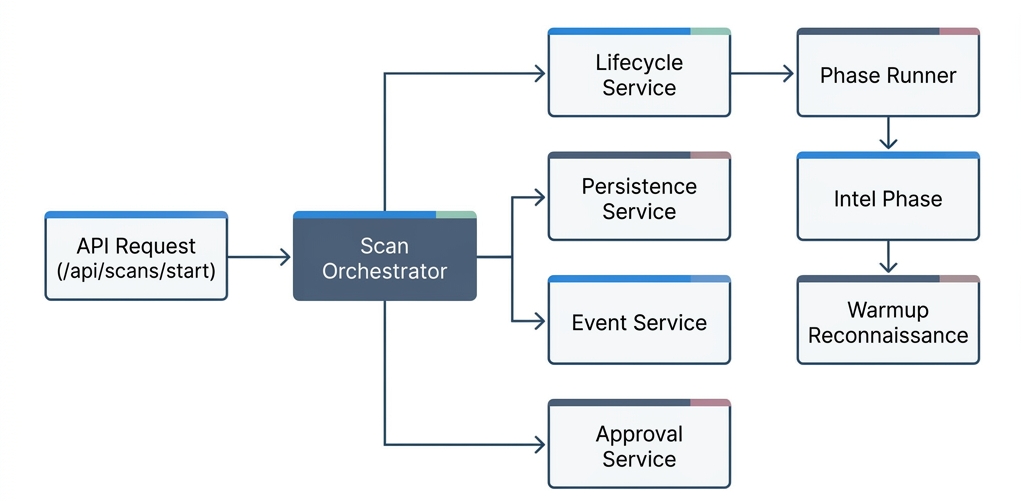
\includegraphics[width=0.75\textwidth]{langgraph_flow.png}
    \caption{Service-based scan flow demonstrating the progression of a run}
    \label{fig:langgraph_flow}
\end{figure}

Operationally, the runner service constructs worker callbacks for the recon lane,
opens analyzer context where needed, and emits structured scan events that are later
consumed by the SSE route. This implementation choice is particularly important from
an engineering standpoint: the frontend is never forced to poll opaque backend state.
Instead, it subscribes to a live stream of scan events that reflect the actual
runtime progression of the platform.

\subsection{Live Observability with Server-Sent Events}

One of the strongest implementation choices of the current project is the use of a
live event stream rather than ad hoc progress polling. The backend exposes
Server-Sent Events (SSE) for scan supervision, and the desktop UI subscribes to this
stream to update dashboards, statuses, approval banners, and activity panels in real
time.

This has two immediate benefits. The first is user experience: the pentester can see
the scan evolve without repeatedly refreshing the interface. The second is
traceability: the same events that feed the UI are persisted or cached as part of the
scan history, which makes later diagnosis easier when a run is interrupted or when a
report must explain the sequence of operations that produced a finding.

\subsection{Data Sanitization and Privacy Layer}

The privacy and safety strategy is implemented as a distributed concern rather than
as a single module. Several layers participate in reducing risk before data reaches
either a language model or an execution path.

\begin{enumerate}
    \item \textbf{API boundary protection:} the backend starts with explicit safety
    middleware that filters requests and centralizes rate-limiting behavior.
    \item \textbf{Prompt path protection:} prompt-guard and privacy-aware services
    reduce the amount of unsafe or irrelevant content introduced into LLM calls.
    \item \textbf{Execution path protection:} run-custom guardrails validate command
    families, target scope, and role compatibility before any action is executed.
    \item \textbf{Delivery protection:} report export and share-link flows support
    password-protected access so that generated outputs remain under operator control.
\end{enumerate}

An important practical result of this implementation is that the same security logic
appears in multiple places with different responsibilities: the API protects entry,
the sandbox protects execution, and the reporting path protects distribution.

\subsection{Analyzer, Findings, and Risk Enrichment}

The analyzer path currently embodies the practical classification engine of the
platform. It receives raw execution outputs, normalizes them, builds summaries,
prepares verification payloads, and persists structured analyzer reports that can be
reused by later reporting and dashboard views.

This implementation is especially visible in two areas:
\begin{itemize}
    \item \textbf{Evidence enrichment:} verified findings are enriched with CVSS
    information before reaching the report generator.
    \item \textbf{Planner handoff:} analyzer results are aggregated and handed back
    into the planning path so that the next execution cycle is based on evidence
    rather than assumptions.
\end{itemize}

The architectural value of this implementation is therefore twofold: it transforms
tool outputs into durable knowledge, and it closes the loop between execution and
planning.

\subsection{RAG Pipeline and Chatbot Interface}

The retrieval path of the implemented project is organized around Qdrant and an Intel
resource model rather than a single ad hoc document collection. The platform stores
target-type-oriented resources, update preferences, and project-level report/finding
artifacts separately, which allows retrieval to serve multiple contexts: planning,
assistant interactions, and reporting.

On the user-facing side, the assistant path is integrated directly into the desktop
experience. The React frontend maintains the conversational state, while the backend
assistant route can access project memory, saved findings, and safe execution tools.
This turns the chatbot into a genuine operator aid rather than a detached natural
language layer.

\subsection{Desktop Workflows and Tauri Integration}

The desktop application is not a thin mockup around the backend. It implements the
operator workflow that gives coherence to the platform: project creation, target-type
selection, scan launch, report review, client delivery, and settings management.
Because the UI is packaged with Tauri, the product preserves the familiarity of a web
interface while remaining distributed as a desktop tool suitable for local use inside
a controlled assessment environment.

From an implementation standpoint, this also simplifies the development rhythm. The
team benefits from the speed of a Vite-based frontend during development, while Tauri
provides the native shell, permissions model, and packaging path required for a
deployable desktop deliverable.

\subsection{Report Generation and Client Delivery}

The reporting path is implemented as a durable backend task. When the operator
requests report generation, the backend creates a report run entry, invokes the
report generator, stores the Markdown report, derives the HTML representation, and
marks the task status as completed or failed. This means that report generation is
traceable in the same way as scan activity.

The delivery path extends this logic. A dedicated share route can create or revoke a
client-facing link, optionally protect it with a password, and expose a scoped
viewer. On the export side, the report module can package protected downloads so that
the generated document does not circulate as an immediately open artifact. This
combination of generation, persistence, and delivery is one of the most concrete
value-producing parts of the platform because it connects raw scan activity to a
usable client deliverable.

\subsection{Target-Type-Aware Configuration}

One of the most distinctive implementation choices of PentaForge is the explicit
modeling of target types. The backend exposes a target-type catalog, dynamic field
extraction from Pydantic schemas, and editable information-gathering profiles. On
the frontend, the project creation dialog consumes this metadata to adapt the data
entry form to the selected target type.

This removes a common source of ambiguity found in generic pentest tools. Instead of
forcing every engagement into a single flat target field, the implementation allows
the project definition itself to carry structured intelligence about web, API,
infrastructure, network, mobile, IoT, cloud, container, repository, and Linux
server targets.

\section{Implementation of the Execution and Safety Path}

\subsection{Dedicated Sandbox Service}

Tool execution is isolated in a dedicated sandbox service exposed over HTTP inside
the Docker environment. The backend does not execute high-risk operational commands
directly in its own process. Instead, it delegates \texttt{run-custom} and
\texttt{run-python} style actions to the sandbox service, which validates the
request, reconstructs the execution context, and performs a second layer of scope
and policy checks.

This design has two major benefits. First, it sharply separates the control plane
from the execution plane. Second, it allows the sandbox image to contain the command
line tooling, wordlists, and execution environment needed by the agents without
inflating the trust placed in the main backend service.

\subsection{Command Guardrails and Resource Resolution}

The sandbox path is coupled with a guard module that classifies tools, detects
recon-role violations, validates network targets against the active scope, and
collects artifact paths created by a command. It also resolves shared resource paths
such as wordlists and SecLists entries into container-friendly locations.

In practice, this means that the implementation does not treat command execution as a
simple shell wrapper. It treats it as a policy-checked action with context, target,
role, and artifact semantics. This is a critical implementation property for a
security product, because the absence of such checks would make the platform itself a
risk.

\subsection{Execution Context and Artifact Handling}

Beyond command validation, the execution lane must also preserve enough context for
results to remain useful after the tool finishes. For that reason, the execution path
transmits identifiers such as project scope, target type, and role semantics together
with the command request. Generated outputs, logs, and evidence paths are then mapped
back to project storage and to the operator-facing reporting path.

This behavior is especially important in an automated penetration testing platform.
Running a tool is not sufficient on its own; the system must also be able to
attribute the output to the right project, the right step of the scenario, and the
right later consumer, whether that consumer is the analyzer, the planner, or the
report generator.

\subsection{Desktop Integration Through Tauri}

On the frontend side, the Tauri shell provides a native desktop container around the
React application. This allows PentaForge to preserve the ergonomics of a modern web
interface while still shipping as a desktop tool. The Tauri configuration defines
the main window, the Vite development workflow, and the production build coupling
between the native shell and the frontend bundle.

This choice is particularly coherent with the product positioning of PentaForge.
Security operators typically prefer locally controlled tools with a desktop
experience, while still expecting rich interactive views, dynamic charts, and
real-time panels. Tauri offers that compromise with lower runtime weight than a full
browser-engine desktop stack.

% ── Section 3 ─────────────────────────────────────────────────────────────
\section{End-to-End Execution on a Test Environment}

To validate the platform in realistic conditions, PentaForge was executed in its
containerized environment with the full operational path enabled: desktop UI,
backend API, Redis, Qdrant, and the isolated tool sandbox. The following scenario
illustrates how the implemented modules cooperate during a standard engagement.

\subsection{Phase 1: Engagement Setup and Project Initialization}

The workflow begins in the Projects page, where the operator creates an engagement,
selects the target type, and fills in the structured target information requested by
the schema for that type. Once the project is saved, the scan can be launched from
the dashboard. The backend immediately registers a runtime state, assigns a scan
identifier, and starts publishing SSE events such as \texttt{scan\_started},
\texttt{intel\_started}, and \texttt{intel\_completed}.

From the operator perspective, this first phase validates two things at once: the
data model is correctly instantiated, and the live observability path is functional.
The frontend does not need to infer progress heuristically; it displays what the
backend explicitly emits.

\begin{figure}[H]
    \centering
    % \includegraphics[width=0.85\textwidth]{ui_dashboard.png}
    \caption{PentaForge Operator Dashboard showing real-time target mapping}
    \label{fig:ui_dashboard}
\end{figure}

\subsection{Phase 2: Intel Preparation and Warmup Reconnaissance}

Once the scan begins, the runner service initializes the Intel node and then the
warmup recon workers. The Intel phase prepares the knowledge baseline of the
engagement, while the information-gathering and recon paths start building the first
usable memory of the target. The recon executers receive scoped target types, tool
availability context, and project-specific execution callbacks. Whenever a tool must
be run remotely, the request is sent to the sandbox service together with the active
execution context.

At this point, the safety path becomes visible in the implementation. Commands are
validated for role and scope compatibility, and any required approval can be surfaced
back to the operator. The result is a supervised execution model: automation is used
to accelerate technical work, but not at the cost of losing operator control.

\subsection{Phase 3: Analysis, Enrichment, and Planning Feedback}

As tool results accumulate, the analyzer path consolidates them into structured
findings and summaries. These outputs are reused in multiple ways: they enrich memory
for later planning, they feed the report generator, and they populate the reporting
surfaces visible to the operator.

This phase is where the circular logic of the platform becomes clear. Execution is
not treated as an end in itself. Each result is interpreted, correlated with
existing memory, and transformed into a planning input for the next step. In other
words, the implementation realizes a genuine feedback loop:
\emph{plan $\rightarrow$ execute $\rightarrow$ analyze $\rightarrow$ update memory
$\rightarrow$ plan again}. This loop is one of the core differentiators of
PentaForge compared with fragmented toolchains in which outputs remain disconnected.

\subsection{Phase 4: Reporting, Export, and Client Delivery}

When report generation is triggered, the backend stores a dedicated report task run,
creates the Markdown report, derives the HTML report, and makes both available in the
Reports page. From there, the operator can preview content, update the Markdown
version when necessary, generate a password-protected export package, or create a
share link for the client portal.

This final phase is especially important because it demonstrates that the project is
not limited to scanning mechanics. It completes the delivery chain: operational
activity is transformed into a reviewable, exportable, and shareable client-facing
artifact.

\begin{figure}[H]
    \centering
    % \includegraphics[width=0.85\textwidth]{ui_report_export.png}
    \caption{Generated finding detail showing evidence capture and SSVC decision}
    \label{fig:ui_report}
\end{figure}

\section*{Conclusion}
\addcontentsline{toc}{section}{Conclusion}

This chapter demonstrated the concrete realization of PentaForge as a working
platform. The architecture described previously was translated into a desktop
application, a FastAPI backend, dedicated scan services, a sandboxed execution lane,
specialized storage components, and a complete reporting and delivery path. Beyond
the individual modules, the implementation also validated a broader design principle:
automation becomes valuable when it is coupled with clear boundaries, explicit
operator control, and durable project state.

By grounding the implementation in real route handlers, service layers, target-type
metadata, SSE observability, report generation, and share-link delivery, the project
demonstrates that PentaForge is not merely a conceptual multi-agent system. It is a
coherent operational platform whose components already interact in a structured and
extensible manner.

% ==================== GENERAL CONCLUSION ====================
\newpage
\thispagestyle{fancy}
\chapter*{General Conclusion}
\addcontentsline{toc}{chapter}{General Conclusion}

The constant evolution of cyber threats, coupled with the exponential growth of organizational 
attack surfaces, has highlighted the structural limitations of traditional, manual 
penetration testing. Organizations require security assessments that are scalable, 
frequent, and highly accurate, without compromising on depth or methodological rigor.

This end-of-studies project, conducted within the cybersecurity team at Talan, aimed to 
solve these challenges through the design and implementation of \textbf{PentaForge}: an 
open-source, AI-powered automated penetration testing platform. 

Throughout this project, we successfully translated complex theoretical concepts into a 
fully functional product. We designed a \textbf{multi-agent architecture} capable of 
orchestrating specialized AI agents (Recon, Exploit, Verify, Report, Retest) to autonomously 
navigate the entire penetration testing lifecycle. We integrated an \textbf{SSVC decision engine} 
to replace static vulnerability scoring with context-aware prioritization. Furthermore, 
we built a persistent \textbf{RAG-powered conversational interface} that bridges the gap 
between raw technical outputs and executive understanding, all while strictly guaranteeing 
the confidentiality of target data through an automated sanitization layer.

From a technical standpoint, this internship was profoundly enriching. It provided an
opportunity to deepen skills in LLM-assisted application design, backend
orchestration with FastAPI and dedicated service layers, and desktop interface
engineering using React and Tauri. The adoption of the Scrum methodology fostered a
professional approach to iterative development, continuous integration, and
stakeholder feedback.

While PentaForge currently represents a powerful enhancement to the pentester's toolkit, 
several perspectives can be explored to expand its capabilities:
\begin{itemize}
    \item \textbf{Integration into CI/CD Pipelines (DevSecOps):} Allowing PentaForge to 
    automatically spawn lightweight agent clusters to test new infrastructure builds 
    before they are merged into production.
    \item \textbf{Continuous Security Validation:} Transitioning from point-in-time scans 
    to a continuous red-teaming mode, where agents persistently monitor the attack surface 
    and react to new CVEs published by the Intel feed in real time.
    \item \textbf{Advanced Privilege Escalation Models:} Enhancing the Exploit Agent
    with richer graph-oriented reasoning and privilege-correlation models to
    autonomously discover complex Active Directory misconfigurations and cross-cloud
    IAM privilege chains.
\end{itemize}

Ultimately, PentaForge demonstrates that artificial intelligence is not meant to replace 
human security experts, nor to independently perform the full work of a penetration 
tester from end to end. Its value lies in serving as a force multiplier: helping 
analysts preserve context, accelerate repetitive operations, and identify potential 
vulnerabilities that must still be interpreted, validated, and prioritized by a human 
professional. By automating the mundane and accelerating the complex, it allows security 
professionals to focus on what truly matters: creative analysis, strategic remediation, 
and staying one step ahead of the adversary.

% ==================== BIBLIOGRAPHY ====================
\cleardoublepage
\addcontentsline{toc}{chapter}{Bibliography}
\begin{thebibliography}{99}

\bibitem{triaxiomTimeline}
Triaxiom Security, \textit{What is the Typical Timeline for a Penetration Test?}, \url{https://www.triaxiomsecurity.com/blog/typical-timeline-for-a-penetration-test/} (accessed 2026).

\bibitem{valuementorLifecycle}
ValueMentor, \textit{Penetration Testing Service Lifecycle}, \url{https://valuementor.com/blogs/penetration-testing-service-inside-the-complete-assessment-lifecycle} (accessed 2026).

\bibitem{autosecagent2026}
AutoSecAgent, \textit{The Journal of Supercomputing} (Springer Nature), 2026, \url{https://link.springer.com/article/10.1007/s11227-026-08439-z}.

\bibitem{emazzantiTools}
eMazzanti Technologies, \textit{Benefits and Limitations of Automated Tools in Penetration Testing}, \url{https://www.emazzanti.net/benefits-and-limitations-of-automated-tools-in-penetration-testing/} (accessed 2026).

\bibitem{pentestgpt2023}
PentestGPT, arXiv:2308.06782, \url{https://arxiv.org/pdf/2308.06782} (accessed 2026).

\bibitem{hedgehogRetesting}
Hedgehog Security, \textit{Remediation Validation and Retesting}, \url{https://www.hedgehogsecurity.co.uk/blog/remediation-validation-retesting-close-the-loop} (accessed 2026).

\bibitem{redleggRetesting}
RedLegg, \textit{The Role of Retesting in Vulnerability Remediation Validation}, \url{https://www.redlegg.com/blog/vulnerability-remediation-retesting-guide} (accessed 2026).

\bibitem{halockVerification}
HALOCK, \textit{Remediation Verification}, \url{https://www.halock.com/penetration-testing/remediation-verification/} (accessed 2026).

\bibitem{cycognitoPentest}
CyCognito, \textit{Penetration Testing} ("Penetration Testing in 2025"), \url{https://www.cycognito.com/learn/penetration-testing/} (accessed 2026).

\end{thebibliography}

\end{document}
